\documentclass[12pt]{article}
\usepackage{amsfonts, amsmath}
\usepackage{amssymb, geometry}
\usepackage{scalefnt}
\usepackage{setspace}
\usepackage{color,hyperref}
%\usepackage{epsfig,subfigure,morefloats}
\usepackage{natbib}
\usepackage{dsfont}
\usepackage{color,hyperref}
\usepackage{epstopdf}
\usepackage{amsthm}
\usepackage{amssymb}
%\usepackage{subcaption}
\usepackage{graphicx}
\usepackage{booktabs,siunitx}
\usepackage{bm}
\usepackage[section]{placeins}
%\usepackage{hypcap}
\usepackage{afterpage}


\setcounter{MaxMatrixCols}{10}

\providecommand{\u}[1]{\protect\rule{.1in}{.1in}}
\providecommand{\u}[1]{\protect\rule{.1in}{.1in}}
\newtheorem{theorem}{Theorem}
\newtheorem{acknowledgement}[theorem]{Acknowledgement}
%\newtheorem{algorithm}[theorem]{Algorithm}
\newtheorem{axiom}[theorem]{Axiom}
\newtheorem{case}[theorem]{Case}
\newtheorem{claim}{Claim}
\newtheorem{conclusion}[theorem]{Conclusion}
\newtheorem{condition}[theorem]{Condition}
\newtheorem{conjecture}{Conjecture}
\newtheorem{corollary}{Corollary}
\newtheorem{criterion}[theorem]{Criterion}
\newtheorem{definition}{Definition}
\theoremstyle{definition}
\newtheorem{example}{Example}
\newtheorem{exercise}{Exercise}
\newtheorem{lemma}{Lemma}
\newtheorem{notation}[theorem]{Notation}
\newtheorem{problem}[theorem]{Problem}
\newtheorem{proposition}{Proposition}
\newtheorem{remark}{Remark}
\theoremstyle{definition}
%\newtheorem{solution}[theorem]{Solution}
\newtheorem{solution}{Solution}
\newtheorem{summary}[theorem]{Summary}
\geometry{left=1in,right=1in,top=1in,bottom=1in}
%\newenvironment{proof}[1][Proof]{\noindent\textbf{#1.} }{\ \rule{0.5em}{0.5em}}
%\hypersetup{pdftex,colorlinks=true,allcolors=black,citecolor=black}

\usepackage{floatrow}
\usepackage{algorithm}
\usepackage{algpseudocode}
\usepackage{float}
\usepackage{indentfirst}

\algnewcommand\algorithmicforeach{\textbf{for each}}
\algdef{S}[FOR]{ForEach}[1]{\algorithmicforeach\ #1\ \algorithmicdo}

\DeclareMathOperator*{\argmax}{arg\,max}
\DeclareMathOperator*{\argmin}{arg\,min}

%\graphicspath{{./Simulation_Graphs/}}

\usepackage{listings}
\usepackage{subcaption} 
\usepackage[toc,page]{appendix}
%\usepackage[extendedchars]{grffile}

\usepackage{mathpazo} % math & rm
\linespread{1.05}        % Palatino needs more leading (space between lines)
\usepackage[scaled]{helvet} % ss
\usepackage{courier} % tt
\normalfont
\usepackage[T1]{fontenc}

%% Math commands
\newcommand{\e}{\epsilon}
%\newcommand{\d}{\delta}
\newcommand{\D}{\Delta}
\newcommand{\R}{\mathbb{R}}
\newcommand{\Z}{\mathbb{Z}}

\setcounter{tocdepth}{4}
%\onehalfspacing

\title{Modern Algebra Lecture Notes}
\author{Rebekah Dix}

\begin{document}
\maketitle
\tableofcontents
\newpage 

\section{Group Theory}
\subsection{Basic Definitions/Examples}
\begin{definition}[Group]
A set $G$ with a binary operation $\star: G \times G \rightarrow G$ is a group if the following axioms are satisfied:
\begin{enumerate} 
\item Associativity: $(a \star b) \star c = a \star (b \star c)$ for every $a,b,c \in G$.
\item Unit (or Identity): There exists an $e \in G$ such that $e \star a = a \star e = a$ for each a in $G$.
\item Inverse: For each $a \in G$ there is a $b \in G$ such that $a \star b = b \star a = e$. 
\end{enumerate} 
\end{definition}

\begin{example}[Examples of Groups] 
The following are examples of groups.
\begin{enumerate}
\item $G = \mathbb{R} \setminus \{ 0 \} = \mathbb{R}^{\star}$ and $\star = $ multiplication. 
\item $G = \mathbb{Z}$ and $\star = $ addition ($e=0$ and $b=-a$).
\item $G = \{ +1, -1 \} \subset \mathbb{R}^{\star}$ and $\star = $ multiplication. 
\item $G = S_3 = \{ \text{ All bijective functions } f: \{1,2,3\} \rightarrow \{1,2,3\} \}$ and $\star = $ composition of functions. To check the axioms in this example:
\begin{enumerate}
\item Associativity: Holds because associativity is a basic property of composition
\item Unit Element: The element that maps 1 to 1, 2 to 2, and 3 to 3 is the unit element. This element moves each element to itself. 
\item Inverse: $S_3$ is the set of bijections, so the definition of bijection implies there is an inverse by composition.
\end{enumerate}
\end{enumerate}
\end{example}

\begin{definition}[Abelian/Commutative]
A group $G$ is abelian or commutative if $a \star b = b \star a$ for all $a \in G$.
\end{definition}

\begin{example}(Examples of Abelian Groups)
\begin{enumerate}
\item Examples 1, 2, and 3 above are Abelian. The commutativity follows from the commutativity of addition and multiplication.
\item Example 4 is not Abelian. It's easy to find a pair of elements that don't commute under composition.
\end{enumerate}
\end{example}

Not everything is a group.
\begin{example}(Non-Examples of Groups)
\begin{enumerate}
\item $G = \mathbb{R}$ and $\star =$ maximum. For example, $2 \star \pi = \max(2,\pi) = \pi$. \underline{Associativity} is satisfied. The order in which we take the maximum of a set of elements doesn't matter -- we'll eventually find the largest element regardless. However, there is no \underline{unit element}. The reason is that there is no smallest element in $\mathbb{R}$.  
\item $G = \mathbb{R}_{\geq 0}$ and $\star =$ maximum. \underline{Associativity} is satisfied. There is a \underline{unit element}, namely $0$ (observe that we've corrected the problem of not having a smallest element). Fix $g \in G$, and observe that $\max(g,0) = \max(0,g) = g$. However, there need not be an \underline{inverse} of each element. We can't take the maximum of some element $g > 0$ and $0$ and get $0$.
\end{enumerate}
\end{example}

\begin{claim}(The unit element is unique)
Let $G$ be a group and $\star$ its binary operation. Suppose that $e_1, e_2 \in G$ are both units elements. Then, $e_1 = e_2$.
\end{claim}
\begin{proof}
Since $e_1$ and $e_2$ are unit elements, we know that for all $a \in G$, $a \star e_1 = e_1 \star a = e_1$ and $a \star e_2 = e_2 \star a = e_2$. Consider the product $e_1 \star e_2$. We know that $e_1 \star e_2 = e_2$ since $e_2$ is a unit element. Further, $e_1 \star e_2 = e_1$ since $e_1$ is a unit element. Therefore, $e_1 = e_2$. 
\end{proof}

\begin{lemma}(Cancellation Law)
For every group $G$ and $a,b,c \in G$ that satisfy $ab = ac$, we have $b=c$.
\end{lemma}
\begin{proof}
Let $x$ be the inverse of $a$. Then, $x(ab) = x(ac)$. Be associativity, we may write $(xa)b = (xa)c$. This simplifies to $1 \star b = 1 \star c$ or that $b = c$.
\end{proof}

\begin{corollary}(The inverse of a group element is unique)
Let $G$ be a group and let $a \in G$. If $b$ and $c$ are inverses of $a$, then $b = c$. 
\end{corollary}
\begin{proof}
Since $b$ and $c$ are inverses of $a$, we know that $ab = 1 = ac$. Then by the Cancellation Law, we know $b=c$.
\end{proof}

\begin{exercise}
Show that if $a,b \in G$, then $(ab)^{-1} = b^{-1}a^{-1}$.
\end{exercise}
\begin{solution} Going back to the definition of a group and the axiom required to be an inverse element, we must show that $(ab)(b^{-1}a^{-1}) = (b^{-1}a^{-1})(ab) = 1$. Then,
\begin{equation}
(ab)(b^{-1}a^{-1}) = a (bb^{-1}) a^{-1} = a \cdot 1 \cdot a^{-1} = aa^{-1} = 1
\end{equation}
And,
\begin{equation}
(b^{-1}a^{-1})(ab) = b^{-1} (a^{-1}a) b = b^{-1} \cdot 1 \cdot b = b^{-1}b = 1
\end{equation}
Therefore, $(ab)(b^{-1}a^{-1}) = (b^{-1}a^{-1})(ab) = 1$ so that $b^{-1}a^{-1}$ is the inverse of $(ab)^{-1}$.
\end{solution}

\begin{exercise}
Give an example of $\tau \in S_3$ such that $\tau \neq 1$, $\tau^2 \neq 1$, and $\tau^3 \neq 1$.
\end{exercise}
\begin{solution}
Consider $\tau(1) = 2$, $\tau(2) = 3$, $\tau(3) = 4$, $\tau(4) = 1$. Then, $\tau^2(1) = 3$ and $\tau^3(1) = 4$. This is sufficient to show that $\tau \neq 1$, $\tau^2 \neq 1$, and $\tau^3 \neq 1$.
\end{solution}

\begin{definition}(The group $\mathbb{Z} / n \mathbb{Z}$)
The group $\mathbb{Z} / n \mathbb{Z}$ is the set $\{0,1,\ldots,n-1\}$. That is, the possible (integer) remainders upon dividing by $n$. Recall that the remainder is the smallest number that you subtract from the original number so that it becomes divisible by $n$. 
\end{definition}
\begin{exercise}
Calculate $5 + 6 + 3$ in $\mathbb{Z} / 7 \mathbb{Z}$.
\end{exercise}
\begin{solution}
$5 + 6+ 3 = 14 = 0$
\end{solution}
\begin{exercise}
What is the inverse of $15$ in $\mathbb{Z} / 30 \mathbb{Z}$.
\end{exercise}
\begin{solution}
Observe that $15 + 15 = 30 = 0$. Hence $15$ is its own inverse.
\end{solution}

\subsubsection{Order}

\begin{definition}(Order of a group, order of an element of a group)
Let $G$ be a group. We call $|G|$ the order of $G$ (i.e. the number of elements in $G$). Further, the least $d >0$ such that $g^d = 1$ is called the order of $g \in G$.
\end{definition}
\begin{example}(Orders of groups)
\begin{itemize}
\item $|S_n| = n!$
\item $|\mathbb{Z} / n \mathbb{Z}| = n$
\end{itemize}
\end{example}

\begin{exercise}
Calculate the order of $2$ in $\mathbb{Z} / 7 \mathbb{Z}$.
\end{exercise}
\begin{solution}
The order of $2$ is $7$.
\end{solution}

\subsubsection{Direct Product}
Given groups $G, H$ we define a group structure on $G \times H$ by $(g_1,h_2)(g_2,h_2) = (g_1g_2,h_1h_2)$. The unit of $G \times H$ is $(1,1) = (1_G, 1_H)$. The inverse of $(g,h)$ is $(g,h)^{-1} = (g^{-1}, h^{-1})$. Questions about direct products will decompose into questions about the individual groups. 

\subsubsection{Symmetric Groups}
\begin{definition}(Cycle, Cycle Decomposition, Length, $k$-Cycle)
A cycle is a string of integers which represents the element of $S_n$ which cyclically permutes these integers (and fixes all other integers). The product of all the cycles is called the cycle decomposition. The length of a cycle is the number of integers which appear in it. A cycle of length $k$ is called a $k$-cycle. 
\end{definition}

\begin{claim}
The order of a $k$-cycle is $k$. 
\end{claim}
\begin{proof}
Let $(i_1 i_2 \ldots i_k)$ be a $k$-cycle. By checking each index, observe that $(i_1 i_2 \ldots i_k)^k = id$. For any $d < k$, note that $(i_1 i_2 \ldots i_k)^d (i_1) = i_{d+1} \neq i_1$, since $d < k$. 
\end{proof}

\begin{claim}
Disjoint cycles commute.
\end{claim}
\begin{proof}
Let $\sigma = (s_1 s_2 \ldots s_k)$ and $\tau = (t_1 t_2 \ldots t_l)$ be disjoint cycles. Consider an index $s_i$ in the first cycle and an index $t_j$ in the second. Then
\begin{equation}
\sigma(\tau(s_i)) = \sigma(s_i) = s_{i+1}
\end{equation}
and
\begin{equation}
\tau(\sigma(s_i)) = \tau(s_{i+1}) = s_{i+1}
\end{equation}
Repeating this argument for all indices shows that
\begin{equation}
\sigma \tau = \tau \sigma
\end{equation}
\end{proof}

\begin{example}
$(2 3 6) (1 4) = (1 4) (2 3 6)$
\end{example}

\subsubsection{Matrix Groups (General Linear Groups)}
\begin{example}
Let $GL_2(\mathbb{R}) = \left\{ \begin{pmatrix} a & b \\ c & d \end{pmatrix} \Big\vert a,b,c,d \in \mathbb{R}, ad-bc \neq 0 \right\}$ and let the binary operation be the multiplication of matrices. Let's check that the axioms are satisfied so that it is a group.
\begin{enumerate}
\item Associativity: Follows from basic properties of matrix multiplication. 
\item Identity: Notice that $\begin{pmatrix} 1 & 0 \\ 0 & 1 \end{pmatrix}$ is the identity element.
\item Inverse: The condition $ad-bc \neq 0$ ensures that each element has an inverse.
\end{enumerate}
For completeness, we also need to check that the product of two invertible matrices is again invertible (one quick proof of this uses the fact that taking a determinant is homomorphism. For instance $\det(A) = \det(A)\det(B)$, From this note that if both $A$ and $B$ have non-zero determinants, then $AB$ also has a non-zero determinant). Also observe that this group is not abelian. More generally, for $n\geq 1$, we can define
\begin{equation}
GL_n(\mathbb{R}) = \left\{ n\times n \text{ matrix } A \Big\vert \det{A} \neq 0 \right\}
\end{equation}
\end{example}

\subsection{Subgroups}
\begin{definition}(Subgroup)
A subset $H$ of a group $G$ is called a subgroup of $G$ if the following axioms are satisfied
\begin{enumerate}
\item Identity: $1 \in H$ (we could also write $1_G \in H$).
\item Closed under products: $h_1 h_2 \in H$ for all $h_1, h_2 \in H$ (in words, the binary operation of $G$ applied to elements of $H$ keeps products in $H$). 
\item Closed under inverses: $h^{-1} \in H$ for all $h\in H$. 
\end{enumerate}
In this case we write $H \leq G$. Observe that $H$ is indeed a group.
\end{definition}

\begin{example}(Examples of Subgroups)
\begin{enumerate}
	\item Define $H = \{ (1 2 3), (1 3 2), id \} \subset S_3$. Let's check the 3 axioms required to be a subgroup.
	\begin{enumerate}
		\item Identity: Observe that $id \in H$.
		\item Closed under products: Define $\sigma = (1 2 3)$. Then $\sigma^2 = (1 3 2)$ and $\sigma^3 = id$. Therefore, $\sigma \circ \sigma^2 = \sigma^3 = id \in H$ and so forth. 
		\item Closed under inverses: Observe that $(1 2 3)^{-1} = (3 2 1) = (1 3 2) \in H$. 
	\end{enumerate}
	\item Define $H = \{ \lambda I_n \vert \lambda \in \mathbb{R} \setminus \{0\} \} \subset GL_n(\mathbb{R})$.
	\begin{enumerate}
		\item Identity: Take $\lambda = 1$.
		\item Closed under products: Fix $\lambda_1, \lambda_2 \in R^{\times}$. Then $(\lambda_1 I)(\lambda_2 I) = (\lambda_1 \lambda_2) I \in H$.
		\item Closed under inverses: Observe that $(\lambda I)^{-1} = \lambda^{-1} I \in H$.
	\end{enumerate}
	\item Define $H = \{2, 4, 0 \} \subset \mathbb{Z} / 6 \mathbb{Z}$.
	\begin{enumerate}
		\item Identity: $0$ is in the set.
		\item Closed under products: Note that $0 + 2 = 2 + 0 = 2 \in H$, $0 + 4 = 4 + 0 = 4 \in H$, and $2 + 4 = 4 + 2 = 0 \in H$.
		\item Closed under inverses: Note that $2^{-1} = 4 \in H$ (because $2 + 4 = 0$) and of course $4^{-1} = 2 \in H$.
	\end{enumerate}
	\item Define $H = \{ \sigma_n \in S_n | \sigma(n) = n \} \subset S_n$ (the set of $n$-permutations which fix the last index).
	\begin{enumerate}
		\item Identity: $id \in H$ because the identity permutation fixes the last element.
		\item Closed under products: Let $\sigma, \tau \in H$. Then $\sigma \circ \tau (n) = \sigma(\tau(n)) = \sigma(n) = n$. Therefore $\sigma \tau$ also fixes the last element.
		\item Closed under inverses: Fix $\sigma \in H$. Since $\sigma$ fixes $n$, it must also be that $\sigma^{-1}$ fixes $n$. In words, $\sigma$ takes $n$ to $n$, so $\sigma^{-1}$ must also take $n$ to $n$.
	\end{enumerate}
\end{enumerate}
\end{example}

\begin{example}(Non-example of Subgroup)
Define $H = \{ \sigma \in S_3 | \sigma(1) \in \{1, 2 \} \} \subset S_3$. 
\begin{enumerate}
	\item Identity: Satisfied.
	\item Closed under products: Consider $\sigma = (1 2 3)$. Then $\sigma^2 = (1 3 2)$. But here, $\sigma(1) = 3$. Therefore this subset is not a subgroup.
\end{enumerate}	
\end{example}

\subsection{Homomorphisms}
\begin{definition}(Homomorphism)
	Let $G, H$ be groups. A function $\phi : G \to H$ is a homomorphism if for every $a,b \in G$, we have 
	\begin{equation}
		\phi(ab) = \phi(a)\phi(b)
	\end{equation}
	Note the the product $ab$ on the left is computed in $G$ and the product $\phi(x)\phi(y)$ is computed in $H$.
\end{definition}

\begin{example}(Examples of Homomorphisms)
\begin{enumerate}
	\item Let $G = GL_n(\mathbb{R})$, $H = \mathbb{R}^{\times}$, $\phi : G \to H$. Define $\phi(A) = \det(A)$.
	\item Let $G = \mathbb{Z} / 7 \mathbb{Z}$, $H = \{z \in \mathbb{C}: z^7 = 1\}$. Define
	\begin{equation}
		\phi(a) = e^{\frac{2\pi i a}{7}}
	\end{equation}
	Then
	\begin{align*}
		\phi(ab) &= \phi(a + b) = e^{\frac{2\pi i (a + b - 7k)}{7}} \\
		&= e^{\frac{2\pi i a}{7}} e^{\frac{2\pi i b}{7}} e^{-2\pi i k}  \\
		&= e^{\frac{2\pi i a}{7}} e^{\frac{2\pi i b}{7}} \cdot 1 \\
		&= \phi(a)\phi(b)
	\end{align*}
	Observe that $\phi$ is injective and surjective. $\phi$ is an isomorphism.
	\item Define $\phi : G \to H$ for all $g \in G$, $\phi(g) = 1$.
	\item Define $\phi : \R^{\times}_{> 0} \to \R$, $\phi(x) = \log(x)$. Then
	\begin{equation}
		\phi(xy) = \log(xy) = \log(x) + \log(y) = \phi(x) \cdot \phi(y) = \phi(x) + \phi(y)
	\end{equation}
\end{enumerate}
\end{example}

\begin{claim}(Basic facts about homomorphisms)
Let $\phi : G \to H$ be a homomorphism. Then
\begin{enumerate}
	\item $\phi(1_G) = 1_H$ (the identity of $G$ is mapped to the identity of $H$).
	\item $\phi(x^{-1}) = \phi(x)^{-1}$ for all $x \in G$.
\end{enumerate}
\end{claim}
\begin{proof}
Observe that
\begin{enumerate}
	\item $1 \cdot \phi(1) = \phi(1) = \phi(1 \cdot 1) = \phi(1)\phi(1)$. Then the (right) cancellation law gives that $1 = \phi(1)$.
	\item $\phi(x^{-1})\phi(x) = \phi(x^{-1}x) = \phi(1) = 1$ and $\phi(x)\phi(x^{-1}) = \phi(xx^{-1}) = \phi(1) = 1$. Therefore, by definition, $\phi(x^{-1}) = \phi(x)^{-1}$.
\end{enumerate}
\end{proof}

\begin{example}(Example of facts about homomorphisms)
Take $\sigma = (1 2 3) \in S_3$. Define $\phi : \mathbb{Z} / 3 \mathbb{Z} \to S_3$ by $\phi(t) = \sigma^t$. Then $\phi(0) = id$ (we expected this from the above claim), $\phi(1) = \sigma$, $\phi(2) = \sigma^2$. 
\end{example}

\begin{claim}
Let $\phi : G \to H$ be a homomorphism. Then $Im(\phi) = \{ \phi(g) | g \in G \} \leq H$.
\end{claim}
\begin{proof}
Let's check the axioms required for $Im(\phi)$ to be a subgroup.
\begin{enumerate}
	\item Identity: Take $1 \in G$, then $\phi(1) = 1 \in Im(\phi)$.
	\item Closed under products: $\phi(a)\phi(b) = \phi(ab) \in Im(\phi)$.
	\item Closed under inverses: $\phi(a)^{-1} = \phi(a^{-1}) \in Im(\phi)$.
\end{enumerate}
Therefore $Im(\phi)$ is a subgroup.
\end{proof}

\begin{example}(The group $n \mathbb{Z}$)
For $n \geq 1$, define $n \mathbb{Z} = \{ k \in \mathbb{Z} : \text{ $k$ is divisible by $n$} \}$. Observe that $n \mathbb{Z} \leq \mathbb{Z}$. Let's check the axioms:
\begin{enumerate}
	\item Identity: $0 \in n \mathbb{Z}$ because $0$ is divisible by everything. 
	\item Closed under products: If $x,y$ are divisible by $n$, then $xy$ will also be divisible by $n$.
	\item Closed under inverses: If $x$ is divisible by $n$, then $-x$ is divisible by $n$.
\end{enumerate}
\end{example}

\begin{example}(Another homomorphism)
Define $\phi : \mathbb{Z} \to \mathbb{Z} / n \mathbb{Z}$ by $\phi(k)$ is the remainder upon dividing $k$ by $n$ (clearly this remainder is in the set $\mathbb{Z} / n \mathbb{Z}$). Then $\phi$ is a homomorphism. We need to show that $\phi(a + b) = a + b$.  

Observations about this example: Note that for each $k \in n \mathbb{Z}$, $\phi(k) = 0$. Moreover $\{ k \in \mathbb{Z} : \phi(k) = 0 \} = n \mathbb{Z}$. This motivates the following definition.
\end{example}

\begin{definition}(Kernel)
Let $\phi:G \to H$ be a homomorphism. Then
\begin{equation}
	\ker(\phi) = \{g \in G : \phi(g) = 1 \}
\end{equation}
(note that $1$ is the identity of H).
\end{definition}

\begin{claim}
Let $\phi: G \to H$ be a homomorphism. Then $\ker(\phi) \leq G$. That is, the kernel of $\phi$ is a subgroup of $G$.
\end{claim}
\begin{proof}
Let's check the 3 axioms required to be a subgroup:
\begin{enumerate}
	\item Identity: Since $\phi$ is a homomorphism, we know that $\phi(1_G) = 1_H$. Therefore $1_G \in \ker(\phi)$.
	\item Closed under products: Let $a,b \in \ker(\phi)$. We want to show that $ab \in \ker(\phi)$, which means that $\phi(ab) = 1$. Then
	\begin{equation}
		\phi(ab) = \phi(a) \phi(b) = 1 \cdot 1 = 1
	\end{equation}
	Therefore $ab \in \ker(\phi)$ so that $\ker(\phi)$ is closed under products. 
	\item Closed under inverses: Let $a \in \ker(\phi)$. Then
	\begin{equation}
		\phi(a^{-1}) = \phi(a)^{-1} = 1^{-1} = 1
	\end{equation}
	Therefore $a^{-1} \in \ker(\phi)$. 
\end{enumerate}
\end{proof}

\begin{example}(Examples of Kernels)
The following are examples of kernels of homomorphisms:
\begin{enumerate}
	\item The determinant is a homomorphism from $GL_n(\mathbb{R})$ to $\R^{\times}$. Then
	\begin{equation}
		\ker(\det) = \{ A \in GL_n(\R) : \det(A) = 1 \}
	\end{equation}
	\item $\phi : S_3 \to \{\pm 1\}$ is a homomorphism. Define $\phi$ as 
	\begin{align*}
		&\phi(1 2 3) = \phi(1 3 2) = 1\\
		&\phi(1 2) = \phi(1 3) = \phi(2 3) = -1 \\
		&\phi(id) = 1
	\end{align*}
	Then $\ker(\phi) = \{(1 2 3), (1 3 2), id \}$.
\end{enumerate}
\end{example}

\subsection{Cosets and Lagrange's Theorem}
\begin{example}(Equivalence Relation)
Let $G$ be a finite group and let $H \leq G$. Define a relation $\sim$ on $G$ by $a \sim b$ if and only if there exists an $h \in H$ such that $a = bh$. This condition also means that $b^{-1}a \in H$. We show that $\sim$ is indeed an equivalence relation:
\begin{enumerate}
	\item Reflexive ($\forall a \in G, a \sim a$): One way to see this is to recall that since $H$ is a subgroup, we know that $a^{-1}a = 1 \in H$. Or simply, $a = a \cdot 1$ and $1 \in H$. 
	\item Symmetric ($\forall a,b \in G, a \sim b \implies b \sim a$): $a \sim b$ implies $b^{-1}a \in H$. We know that then $(b^{-1}a)^{-1} = a^{-1}b \in H$. Therefore $b \sim a$. 
	\item Transitive ($\forall a,b,c \in G, a \sim b, b\sim c \implies a \sim c$): $a \sim b$ implies $b^{-1}a \in H$ and $b \sim c$ implies $c^{-1}b \in H$. $H$ is a subgroup, so it's closed under products. Thus $c^{-1}bb^{-1}a \in H$ or that $c^{-1}a \in H$. Therefore $a \sim c$.
\end{enumerate}
Then let $[a] = \{ b \in G | b \sim a \} = \{b \in G | \exists h \in H, b = ah \} = \{ah | h \in H \} = aH$. $G$ can be written as a disjoint union of equivalence classes. 
\end{example}

\begin{definition}(Coset)
Let $H \leq G$ and fixed $a \in G$. Let
\begin{align*}
aH &= \{ ah | h \in H \} \\
Ha &= \{ ha | h \in H \} 
\end{align*}
These sets are called a left coset and right coset of $H$ in $G$. 

Write $G/H$ for the set of left cosets $\{aH | a \in G \}$.
\end{definition}

\begin{example}(Cosets)
If $a=1$, then $aH = 1 \cdot H = H$. And, for any $a \in H$, $aH = H$: First observe that $aH \subset H$ since $H$ is a subgroup. Indeed if $a,h \in H$, then $ah \in H$. Next we'll show $H \subset aH$. Fix $h \in H$. We want to show that $h \in aH$, or that it can written in the form $a'h'$ where $h' \in H$. To achieve this, write $h = e \cdot h = a (a^{-1} h)$. Note that $a^{-1} h \in H$ since $H$ is a subgroup. Therefore $h \in aH$. Together these equivalences show that $aH = H$ when $a \in H$. 
\end{example}

\begin{claim}(All left cosets of $H$ have the same size) 
Let $H \leq G$ be groups and let $a \in G$. Then $|[a] | = |aH| = |H|$
\end{claim}
\begin{proof}
We can give a bijection between the two sets to show they have the same number of elements. To that end, define $f: H \to aH$ by $f(h) = ah$. 
\begin{enumerate}
	\item $f$ is injective: Fix $h_1, h_2 \in H$ such that $f(h_1) = f(h_2)$. Then $a h_1 = a h_2$. Use the left cancellation law see that $h_1 = h_2$. 
	\item $f$ is surjective: We need to show that for all $h' \in aH$ there exists an $h \in H$ such that $f(h) = h'$. Consider $h = a^{-1} h'$. Then $f(a^{-1} h') = a a^{-1} h' = h'$. 
\end{enumerate}
Thus $f$ is a bijection. This result of course implies that $|aH| = |bH| = |H|$ for all $a, b \in H$. In words, all left cosets of $H$ have the same size as $H$. 
\end{proof}

\begin{theorem}(Lagrange)
	Let $G$ be a finite group and let $H \leq G$. Then $|H|$ divides $|G|$.
\end{theorem}

\begin{proof}
Using the above claim, define $f : H \to aH$ by $f(h) = ah$. Then it follows that $|[a] | = |aH| = |H|$. We can write $G$ as a disjoint union of equivalence classes. Let $k$ be the number of equivalence classes, and observe that they all have the same cardinality of as $H$. Therefore $|G| = k \cdot |H|$, so that $|H| \big\vert |G|$.
\end{proof}

\begin{definition}(Index)
If $G$ is a group (possibly infinite) and $H \leq G$, the number of left cosets of $H$ in $G$ is called the index of $H$ in $G$ and is denoted by $|G : H|$. Alternatively, $|G : H| = | G / H | =  |\{aH | a \in G\} |$. If $G$ is finite, the $|G:H| = \frac{|G|}{|H|}$.
\end{definition}

\begin{example}(Index when $G$ finite)
Let $G = S_3$ and $H = \{ (1 2 3), (1 3 2), id \}$. $H$ is a subgroup. Since $G$ is finite, we can calculate the index of $H$ in $G$ as
\begin{equation}
	|G : H| = \frac{|G|}{|H|} = \frac{6}{3} = 2
\end{equation}
Thus there are $2$ left cosets of $H$ in $G$. To write out $G/H$ we need only find one other left coset other than the trivial coset. To do this, we can pick an element of $G$ that is not in $H$. Then observe that 
\begin{equation}
	G/H = \{H, (1 2) H \}
\end{equation}
You can verify that $(1 2) H = (1 3) H = (2 3) H$.
\end{example}

\begin{example}(Index when $G$ infinite)
$\mathbb{R}_{>0} \subset \mathbb{R}^{\times}$. Then $|\mathbb{R}^{\times} : \mathbb{R}_{> 0}| = 2$. Recall that this means that there are two left cosets of $\mathbb{R}_{>0}$ in $\mathbb{R}^{\times}$. We can enumerate these as follows
\begin{equation}
	\mathbb{R}^{\times} / \mathbb{R}_{> 0} = \{\mathbb{R}_{> 0}, (-1) \cdot \mathbb{R}_{> 0}\}
\end{equation}
We can make an observation about the left cosets of $\mathbb{R}_{> 0}$ more generally:
\begin{equation}
	a \mathbb{R}_{> 0} = sgn(a) \cdot \mathbb{R}_{> 0}
\end{equation}
\end{example}

\begin{example}(Index of Permutation Group)
As a slight abuse of notation, let $S_3$ be the set of permutations in $S_4$ for which the last index is fixed. Then, since $S_3$ is finite
\begin{equation}
 	|S_4 : S_3| = \frac{24}{6} = 4
\end{equation} 
Therefore $S_4 / S_3$ has 4 elements. To find the left cosets of $S_3$ in $S_4$, look for elements of $S_4$ that aren't in $S_3$. Intuitively, these are the permutations that \textit{don't} fix 4. We can enumerate the left cosets as
\begin{enumerate}
	\item $C_1 = \{\sigma \in S_4 | \sigma(4) = 4 \}$ (this is the trivial coset)
	\item $C_2 = \{\sigma \in S_4 | \sigma(4) = 3 \}$
	\item $C_3 = \{\sigma \in S_4 | \sigma(4) = 2 \}$
	\item $C_4 = \{\sigma \in S_4 | \sigma(4) = 1 \}$
\end{enumerate}
Note that we can write each of these cosets as (using $C_2$ as an example): $\tau S_3$, where $\tau(4) = 3$. We can pick any such $\tau$ that satifies this requirement, and the left cosets generated by the different choices of $\tau$ will be the same.
\end{example}

\begin{definition}(Normal Subgroup)
We say that a subgroup $H$ of $G$ is normal if $aH = Ha$ for every $a \in G$. Write $H \trianglelefteq G$. This means that the left and right cosets of a group of equivalent.
\end{definition}

\begin{example}(Non-example of a Normal Subgroup)
Continuing the above example, let $S_3$ be the set of permutations in $S_4$ for which the last index is fixed [[Incomplete]].
\end{example}

\begin{claim}(The Kernal of a Homomorphism is a Normal Subgroup)
Let $\phi : G \to H$ be homomorphism. Then $\ker (\phi) \trianglelefteq G$.
\end{claim}
\begin{proof}(Easier Proof)
We've already shown that $\ker \phi$ is a subgroup of $G$. To show that it is a normal subgroup, we will show that $g k g^{-1} \in \ker \phi$ for all $g \in G$ and $k \in \ker \phi$. This is equivalent to showing that $\phi(g k g^{-1}) = 1$ for all $g \in G$ and $k \in \ker \phi$. Then
\begin{align*}
	\phi(g k g^{-1}) &= \phi(g)\phi(k)\phi(g^{-1}) \\
	&= \phi(g) \phi(g)^{-1} \\
	&= 1
\end{align*}
Therefore $g k g^{-1} \in \ker \phi$ for all $g \in G$ and $k \in \ker \phi$, so that $\ker \phi$ is a normal subgroup of $G$. 
\end{proof}

\begin{proof}(Harder Proof)
We will show that for all $a \in G$, 
\begin{equation}
	a \ker\phi = \{g \in G | \phi(g) = \phi(a) \} = \ker \phi a
\end{equation}
Let $S = \{g \in G | \phi(g) = \phi(a) \}$ and fix and $a \in G$. 

Let $at \in a \ker \phi$. Then 
\begin{equation}
	\phi(at) = \phi(a)\phi(t) = \phi(a)
\end{equation}
Thus $a \ker \phi \subset S$. 

Next let $g \in S$. Therefore $\phi(g) = \phi(a)$, so that $\phi(a^{-1}) \phi(g) = 1 = \phi(a^{-1}g)$. Therefore $a^{-1}g \in \ker \phi$, so that $S \subset a \ker\phi$. 

The proof for the right cosets is similar. Together, these inclusions show that $\ker \phi$ is a normal subgroup. 
\end{proof}

\subsection{Cyclic Groups}
\begin{definition}(Cyclic Group)
A group $H$ is cyclic if $H$ can be generated by a single element, i.e., there is some element $x \in H$ such that $H = \{x^n | n \in \mathbb{Z} \}$. Write $H  = \langle x \rangle$ and say $H$ is generated by $x$.

An alternative definition is: Let $G$ be a group and fix $x \in G$. Let $H$ be the subset of $G$ that contains all the powers of $x$. Then notice that $H = \{x^n | n \in \mathbb{Z} \}$ is a subgroup of $G$ (the identity element must be in $H$ since $x^0 = 1$, $H$ is closed under products since adding exponents will keep us in $H$, and the inverse of $x^n$ is $x^{-n}$, which is also in $H$). We call $H$ the subgroup of $G$ generated by $x$, $H = \langle x \rangle$, and $H$ is cyclic.  
\end{definition}

\begin{example}(Examples of Cyclic Groups)
\begin{enumerate}
	\item Let $x = \begin{pmatrix} 1 & 1 \\ 0 & 1 \end{pmatrix} \in GL_2(\mathbb{R})$. Then
	\begin{equation}
		\langle x \rangle = \left\{ \begin{pmatrix} 1 & n \\ 0 & 1 \end{pmatrix} \Big\vert n \in \mathbb{Z} \right\}
	\end{equation}
	You can see that taking positive powers of $x$ continually increases the element in the upper-right hand corner. Finally, observe that 
	\begin{equation}
		x^{-1} = \begin{pmatrix} 1 & -1 \\ 0 & 1 \end{pmatrix}
	\end{equation}
	Therefore the powers of the inverse of $x$ are also included in $\langle x \rangle$.
	\item Let $x = 3 \in \mathbb{Z} / 6 \mathbb{Z}$. Then $\langle x \rangle = \{ 0, 3 \}$.
\end{enumerate}
\end{example}

\begin{claim}(Every cyclic group is isomorphic to either $\mathbb{Z}$ or to $\mathbb{Z} / n \mathbb{Z}$ for some $n \geq 1$.) For every group $H$ for which there exists an $x \in H$ such that $H = \langle x \rangle$, there exists a bijective homomorphism (i.e. an isomorphism) $\phi : H \to C$ where $C = \mathbb{Z}$ or $C = \mathbb{Z} / n \mathbb{Z}$ for some $n \geq 1$.
\end{claim}
\begin{proof}
There are two cases to consider. 
\begin{enumerate}
	\item The powers of $x$ are distinct: Define $\phi : H \to \mathbb{Z}$ by $\phi(x^n) = n$. $\phi$ is bijective by construction. To check that $\phi$ is indeed a homomorphism, observe that
	\begin{equation}
		\phi(x^n \cdot x^m) = \phi(x^{n+m}) = n + m = \phi(x^n) + \phi(x^m)
	\end{equation}
	\item The powers of $x$ are not distinct: Suppose there is some $m \neq n$ such that $x^m = x^n$ (without loss of generality assume $m \leq n$). Then since $x^m = x^n$, we find that $x^m x^{-m} = x^n x^{-m}$. Therefore $x^{n-m} = 1$. Since there is some finite power of $x$ that equals the identity, let $k$ be the order of $x$. Define $\phi : H \to \mathbb{Z} / k \mathbb{Z}$ by $\phi(x^m) = r$, where $r$ is the remainder upon dividing $m$ by $k$. Surjectivity is clear by definition. To show $\phi$ is injective, we can use the fact that since $\phi$ is a homomorphism, it is injective if and only if $\ker{\phi} = 1$. Then
	\begin{align*}
		\ker{\phi} &= \{x^r : \phi(x^r) = 0 \} \\
		&= \{x^r : k \text{ divides } r \} \\
		&= \{x^{kt} : t \in \Z \} \\
		&= \{ 1 \} \tag{since $k$ is the order of $x$}
	\end{align*}
\end{enumerate}
\end{proof}

\begin{claim}
Let $G$ be a finite cyclic group of order $n$. For every $m | n$ ($m$ that divides $n$) there exists a unique subgroup $H$ of $G$ with $|H|=m$. Furthermore, $H$ is cyclic.
\end{claim}
\begin{proof}
Assume that $G = \mathbb{Z} / n \mathbb{Z}$. This is without generality since $G$ is a finite cyclic group, and every finite cyclic group is isomorphic to $\mathbb{Z} / n \mathbb{Z}$. Definite $H = \langle \frac{n}{m} \rangle$, Indeed, $H = \{ 0, \frac{n}{m}, \frac{2n}{m}, \ldots, \frac{(m-1)n}{m} \}$, and $|H| = m$. 
\end{proof}

\subsection{Dihedral Groups}
For each $n \geq 3$, let $D_n$ be the set of symmetries of the regular $n$-gon. A symmetry is a rigid motion of the $n$-gon which takes a copy of the $n$-gon, moves this copy through space, and places the copy back on the original $n$-gon so it exactly covers it.  

In general, we consider two types of symmetries:
\begin{enumerate}
	\item Rotational symmetries (denoted $\rho$)
	\item Mirror symmetries (denoted by $\e$). There is a distinction in the mirror symmetries when $n$ is even and when $n$ is odd. When $n$ is odd, the mirror symmetries (i.e. the line of symmetry in this case) all have the same form of starting from a vertex and going to the mid-point of the edge opposite of the vertex. When $n$ is even, the lines of symmetry either go from a vertex to a vertex or from a mid-point of an edge to the mid-point of an edge. 
\end{enumerate}
For a regular $n$-gon, there are $n$ rotational symmetries and $n$ mirror symmetries. Therefore $|D_n| = 2n$.

\begin{example}($D_3$, Symmetries of a Triangle)
\begin{figure}[H]
	\begin{center}
		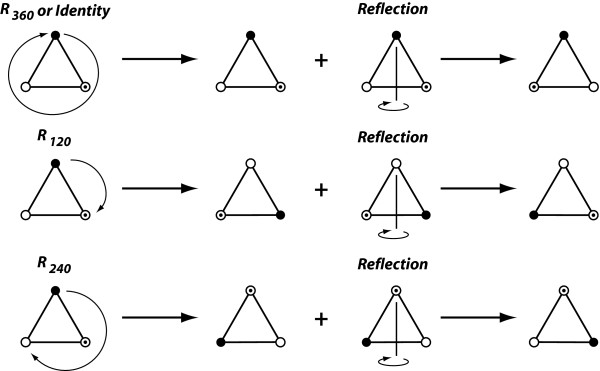
\includegraphics[scale=3]{triangle_symmetries}
	\end{center}
	\caption{The symmetries of an equilateral triangle}
	\label{triangle_sym}
\end{figure}
\end{example}

\begin{example}($D_4$, Symmetries of a Square)
\begin{figure}[H]
	\begin{center}
		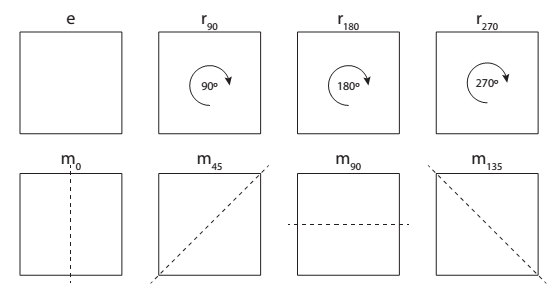
\includegraphics[scale=.75]{square-symmetries}
	\end{center}
	\caption{The symmetries of a square}
	\label{triangle_sym}
\end{figure}

\end{example}

\begin{definition}(Dihedral Group, $D_n$)
In general, $D_n$ is a group with $2n$ elements, where the binary operation is composition. It contains two types of symmetries:
\begin{enumerate}
	\item The rotation $\rho$ is $\frac{2\pi}{n}$ radians clockwise. The set of all rotations is $\langle \rho \rangle = \{1, \rho, \rho^2, \ldots, \rho^{n-1} \}$. 
	\item Let $\e$ be a vertical mirror symmetry. Then the set of all mirror symmetries is $\{\e, \e\rho, \e\rho^2, \ldots, \e \rho^{n-1} \}$. 
\end{enumerate}
\end{definition}


\begin{claim}(Important Identity)
$\rho \e = \e \rho^{-1}$. 
\end{claim}
We use this relation to make computations in dihedral groups. 


\begin{claim}
$\rho^i \e = \e \rho^{-i}$
\end{claim}
\begin{proof}
By induction, using the above claim. 
\end{proof}

\begin{example}(Uniqueness of rotations/mirror symmetries)
Can two elements in the mirror symmetry set be equal, or equal to an element in the set of rotations? No! Suppose $\e \rho^i = \e \rho^j$. Then $\rho^i = \rho^j$, which implies $i = j$. Now suppose $\e \rho^i = \rho^j$, which implies $\e = \rho^{j-i}$. However this implies $\e$ is a rotation, which is nonsense.
\end{example}

\begin{example}(Mirror Symmetries are a Coset)
Observe that the set of mirror symmetries is simply $\e \langle \rho \rangle$, thus they are a left coset of the cyclic group of rotations.  Then
\begin{equation}
	D_n / \langle \rho \rangle = \{ \langle \rho \rangle, \e \langle \rho \rangle\}
\end{equation}
Since $|D_n| = 2n$ and $|\langle \rho \rangle| = n$, we know that by Lagrange's theorem, $[D_n : \langle \rho \rangle] = 2$. 
\end{example}

\begin{example}
In $D_5$, compute (simplify)
\begin{equation}
\rho \e^7 \rho \e \rho^2 \e \rho^{-3} \e^{-1}
\end{equation}
We know that $\rho \e = \e \rho^{-1}$, $\rho^5 = 1$, and $\e^2 = 1$. Then, with the strategy of pushing $\e$ to the left,
\begin{align*}
	\rho \e^7 \rho \e \rho^2 \e \rho^{-3} \e^{-1} &= \rho \e \rho \e \rho^2 \e \rho^{2} \e \tag{$\rho^{-3} = \rho^{2}, \e^{-1} = \e$} \\
	&= \rho \e \rho \e \rho^2 \e \rho \e \rho^{-1} \\
	&= \rho \e \rho \e \rho^2 \e \e \rho^{-1} \rho^{-1} \\
	&= \rho \e \rho \e \rho^2 \rho^{-1} \rho^{-1} \\
	&= \rho \e \rho \e \\
	&= \rho \e \e \rho^{-1} \\
	&= 1
\end{align*}
\end{example}

\subsection{Quotient Groups}

\begin{definition}(Quotient Group)
Let $G$ be a group and $N \trianglelefteq G$ (that is, $N$ is a normal subgroup of $G$). Let $G/N = \{gN|g \in G\}$ be the set of left cosets of $N$ in $G$. Then the quotient group of $G$ by $N$ is the group $(G/N, \cdot)$, where $\cdot$ is the binary operation on $G/N$ defined for all $g_1 N, g_2 N \in G / N$ by $g_1 N g_2 N = g_1g_2N$. 
\end{definition}

\begin{claim}
In the above definition, $G/N$ is a group. 
\end{claim}
\begin{proof}
Binary operation well-defined: We need to check that $\cdot: G/N \times G/N \to G/N$, where $(g_1N, g_2N) \to g_1 g_2 N$ is well-defined (A function is well-defined if it gives the same result when the representation of the input is changed without changing the value of the input. In this context, we show that the definition of multiplication depends on only the cosets and not on the coset representatives). Suppose that $g_1 N = g'_1 N$ and $g_2 N = g'_2 N$, so we want to show $g_1 g_2 N = g'_1 g'_2 N$. Then $g_1N = g'_1 N \iff (g'_1)^{-1} g_1 \in N$ and $g_2 N = g'_2 N \iff (g'_2)^{-1} g_2 \in N$. We then want to show $(g'_1g'_2)^{-1}g_1g_2 \in N$. Then
\begin{align*}
	(g'_1g'_2)^{-1}g_1g_2 &= (g'_2)^{-1} (g'_1)^{-1} g_1 g_2 \\
	&= (g'_2)^{-1} n g_2 \tag{$n = (g'_1)^{-1} g_1 \in N$} \\
	&= (g'_2)^{-1} n g'_2 (g'_2)^{-1} g_2 \\
	&= (g'_2)^{-1} n g'_2 n' \tag{$n' = (g'_2)^{-1} g_2 \in N$}\\
	&= (g'_2)^{-1} g'_2 n'' n' \tag{$N$ is normal}\\
	&= n'' n' \in N
\end{align*}
Therefore the binary operation is indeed well-defined. 

We now check the axioms required to be a group.

\begin{enumerate}
	\item Identity: Observe that
	\begin{equation}
		1 \cdot N = N
	\end{equation}

	\item Inverse: Observe that
	\begin{equation}
		(gN)^{-1} = g^{-1}N
	\end{equation}
	because 
	\begin{equation}
		gNg^{-1}N = gg^{-1} N = N
	\end{equation}

	\item Associativity: Follows clearly from the associativity of $G$. 
	\begin{align*}
		(g_1 N g_2 N)(g_3 N) &= (g_1 g_2 N)(g_3 N) \\
		&= g_1 g_2 g_3 N \\
		&= (g_1 N) (g_2 g_3 N) \\
		&= (g_1 N)(g_2 N g_3 N)
	\end{align*}
\end{enumerate}

Therefore $G/H$ is a group. 
\end{proof}

\begin{example}(Examples of Quotient Groups)
\begin{enumerate}
	\item $\mathbb{R}^{\times} / \mathbb{R}_{> 0} = \{\mathbb{R}_{> 0}, (-1) \cdot \mathbb{R}_{> 0}\} \cong \{\pm 1\}$
	\item $\mathbb{Z} / 12 \mathbb{Z} = \{0 + 12 \mathbb{Z}, 1 + 12 \mathbb{Z}, \ldots, 11 + 12 \mathbb{Z} \} $
	\item $(\mathbb{Z} / 12 \mathbb{Z}) / \{0, 4, 8 \} \cong \mathbb{Z} / 4 \mathbb{Z}$. Thus this quotient group has $4$ elements (we can also see this from Lagrange's theorem). Also observe that this is a cyclic group.
\end{enumerate}
\end{example}

\subsection{Isomorphism Theorems}

\begin{theorem}(The First Isomorphism Theorem)
If $\phi:G\to H$ is a homomorphism of groups, then $G / \ker(\phi) \cong Im \phi$. 
\end{theorem}

\begin{proof}
Define $f: G / \ker(\phi) \to Im \phi$ by $f(a \ker(\phi)) = \phi(a)$. We first show $f$ is indeed well-defined. To that end, pick $a \ker(\phi) = b \ker(\phi)$. Therefore there exists some $k \in \ker(\phi)$ such that $a = bk$. Then
\begin{equation}
	\phi(a) = f(a \ker(\phi)) = f(bk \ker(\phi)) = f(b \ker(\phi)) = \phi(b)
\end{equation}
Therefore $f$ is well-defined. We now show $f$ is an isomorphism. 

\begin{enumerate}
	\item $f$ is a homomorphism: 
	\begin{align*}
		f(a \ker(\phi) b \ker(\phi)) &= f(ab \ker(\phi)) \\
		&=  \phi(ab) \\
		&= \phi(a)\phi(b) \tag{$\phi$ is a homomorphism} \\
		&= f(a \ker(\phi)) f(b \ker(\phi))
	\end{align*}

	\item $f$ is surjective: Let $\phi(a) \in Im \phi$. Then $f(a \ker \phi) = \phi(a)$. 
	\item $f$ is injective:  
	\begin{align*}
		\ker(f) &= \{a \ker \phi : f(a \ker \phi) = 1_H \} \\
		&= \{a \ker \phi : \phi(a) = 1_H \} \\
		&= \{\ker \phi \} 
	\end{align*}
	Thus the kernal of $f$ is trivial (the trivial left coset), so $f$ is injective. 
\end{enumerate}

Therefore $f$ is an isomorphism.
\end{proof}

Intuition for this theorem:
\begin{itemize}
	\item This is a more general version of the rank-nullity theorem.
	\item Given vector spaces $V, W$ and a linear transformation $A : V \to W$, this theorem says
	\begin{equation}
		dim( V / \ker A ) = dim (range(A))
	\end{equation}
	or that
	\begin{equation}
		dim(V) - nullity(A) = rank(A)
	\end{equation}
\end{itemize}

\begin{example}(Examples of applications of first isomorphism theorem) Consider the following examples
\begin{enumerate}
	\item $sgn : \R^{\times} \to \{\pm 1 \}$. This is indeed a homomorphism. By the theorem, we know that
	\begin{equation}
		\R^{\times} /\ker(sgn) \cong \{ \pm 1\}
	\end{equation}
	Then $\ker(sgn) = \R_{>0}$. This matches the previous example. 
	\item $\det : GL_2(\mathbb{R}) \to \R^{\times}$. The theorem implies
	\begin{equation}
		GL_2(\mathbb{R}) / \{A \in GL_2(\mathbb{R}) | \det(A) = 1 \} \cong \R^{\times}
	\end{equation}
\end{enumerate}

\end{example}

\begin{theorem}(The Second or Diamond Isomorphism Theorem)
Let $H \leq G$ and $K \trianglelefteq G$. Then $HK / K \cong H / H \cap K$. 
\end{theorem}

\begin{proof}
Define $f : HK / K \to H / H \cap K$ by 
\begin{equation}
	f(hk K) = h (H \cap K)
\end{equation}
We'll first show $f$ is well-defined. Fix $hk, h'k' \in HK$ such that $hk K = h'k'K \in HK/K$. There $h = h'\tilde{k}$ for some $\tilde{k} \in K$. Then
\begin{equation}
	h (H \cap k) = f(hk K) = f(h' \tilde{k} K) = h' (H \cap K)
\end{equation}
Therefore $f$ is well-defined, and we now show $f$ is an isomorphism.
\begin{enumerate}
	\item $f$ is a homomorphism:
	\begin{align*}
	f(h_1 k_1 K \cdot h_2 k_2 K) &= f(h_1 K \cdot h_2 K) \\
	&= f(h_1h_2 K) \\
	&= h_1h_2 (H \cap K) \\
	&= h_1 (H \cap K) h_2 (H \cap K) \\
	&= f(h_1 k_1 K) f(h_2 k_2 K)
	\end{align*}
	\item $f$ is surjective: Clear by the definition of $f$. 
	\item $f$ is injective: We'll show the kernal of $f$ is trivial (in this context, the trivial left coset). 
	\begin{align*}
		\ker(f) &= \{ hk \cdot K | f(hk \cdot K) = H \cap K \} \\
		&= \{ hk \cdot K | h (H \cap K) = H \cap K \} \\
		&= \{ hk \cdot K | h \in H \cap K \} \tag{$h (H\cap K) = H \cap K \iff h \in H\cap K$} \\
		&= \{K \}
	\end{align*}
\end{enumerate}
\end{proof}

\section{Quizzes}
The course did not give solutions to any quizzes, homeworks, or midterms, so be wary of the solutions I've written below. 

\subsection{Quiz 1}

\begin{exercise}
Give an example of $\sigma \in S_3$ such that $\sigma$ has order 3. 
\end{exercise}
\begin{solution}
Consider $\sigma = (1 2 3)$. Then $\sigma^2 = (1 3 2)$ and $\sigma^3 = (1)(2)(3)$. Therefore, $\sigma^1 \neq 1$, $\sigma^2 \neq 1$, but $\sigma^3 = 1$. Therefore, by definition, $\sigma$ has order $3$.
\end{solution}

\begin{exercise}
Give an example of $\tau \in S_5$ such that $\tau$ has order 6. 
\end{exercise}
\begin{solution}
Consider $\tau = (123)(45)$. Then $\tau^2 = (132)(4)(5)$, $\tau^3 = (1)(2)(3)(45)$, $\tau^4 = (123)(4)(5)$, $\tau^5 = (132)(45)$, $\tau^6 = (1)(2)(3)(4)(5)$.
\end{solution}

\subsection{Quiz 2}
\begin{exercise}
Let $\tau \in S_6$. Show that
\begin{equation*}
\tau \cdot (5 4 1 3 2) \cdot \tau^{-1} = (\tau(5) \tau(4) \tau(1) \tau(3) \tau(2))
\end{equation*}
\end{exercise}

\begin{solution}
We can show this element by element. Observe that
\begin{equation}
	\tau \cdot (54132) \cdot \tau^{-1}(\tau(5)) = \tau \cdot (54132)(5) = \tau(4)
\end{equation}
This shows that $\tau \cdot (54132) \cdot \tau^{-1}$ maps $\tau(5)$ to $\tau(4)$. Similarly,
\begin{align}
&\tau \cdot (54132) \cdot \tau^{-1}(\tau(4)) = \tau \cdot (54132)(4) = \tau(1) \\
&\tau \cdot (54132) \cdot \tau^{-1}(\tau(1)) = \tau \cdot (54132)(1) = \tau(3) \\
&\tau \cdot (54132) \cdot \tau^{-1}(\tau(3)) = \tau \cdot (54132)(3) = \tau(2) \\
&\tau \cdot (54132) \cdot \tau^{-1}(\tau(2)) = \tau \cdot (54132)(2) = \tau(5) 
\end{align}
Therefore $\tau \cdot (5 4 1 3 2) \cdot \tau^{-1} = (\tau(5) \tau(4) \tau(1) \tau(3) \tau(2))
$.
\end{solution}		

\begin{exercise}
Let $G$ be a group and fix $g \in G$. Define $\phi : G \to G$ by $\phi(x) = gxg^{-1}$. Show $\phi$ is an isomorphism.
\end{exercise}
\begin{solution}
\begin{enumerate}
	\item $\phi$ is a homomorphism: Fix $x, y \in G$. Then
	\begin{align*}
	\phi(xy) &= g (xy) g^{-1} \\
	&= g x g^{-1} g y g^{-1} \\
	&= \phi(x) \phi(y)
	\end{align*}
	\item $\phi$ is injective: Fix $x, y \in G$, and suppose $\phi(x)=\phi(y)$. Then
	\begin{equation}
		\phi(x) = g x g^{-1} = g y g^{-1} = \phi(y) 
	\end{equation}
	Then use the right and left cancellation laws we get that $x = y$.
	\item $\phi$ is surjective: Fix $y \in G$ and consider $x = g^{-1} y g$. Then
	\begin{equation}
		\phi(g^{-1}yg) = g (g^{-1}yg) g^{-1} = y
	\end{equation}
	Therefore, for all $y \in G$, we can find an $x = g^{-1} y g$ such that $\phi(x) = y$.
\end{enumerate}
\end{solution}

\subsection{Quiz 3}
\begin{exercise}
Let $G$ be a group and define $\phi : G \to G$ by $\phi(g) = g^{-1}$ for $g \in G$. Show that $\phi$ is a homomorphism if and only if $G$ is abelian.
\end{exercise}
\begin{solution}

\end{solution}

\begin{exercise}
Define $H = \{\sigma \in S_5 : \{\sigma(1), \sigma(2), \sigma(3) \} \in \{ 1, 2, 3 \} \}$. Show that $H \leq S_5$ and calculate $[S_5 : H]$. 
\end{exercise}
\begin{solution}

Since $S_5$ is a finite group, we can use Lagrange's theorem to find $[S_5 : H] = \frac{|S_5|}{|H|}$.  $|S_5| = 5! = 120$. Then $|H| = 3! \times 2! = 12$. Therefore 
\end{solution}

\section{Exams}
\subsection{Exam 1}

\section{Homework Exercises}
\subsection{Homework 1}
\begin{exercise}
Show that the group $S_3$ is not abelian. 
\end{exercise}
\begin{solution}
To show that $S_3$ is not abelian, we must find an $a,b \in S_3$ such that $ab \neq ba$. To this end, consider the permutations $a(1) = 2, a(2) = 3, a(3) = 1$ and $b(1) = 1, b(2) = 3, b(2) = 2.$ Then, $a(b(1))= 2$ but $b(a(1)) = 3$. Therefore, $ab \neq ba$, so $S_3$ is not abelian.
\end{solution}

\begin{exercise}
Is the set $\mathbb{R}$ of real numbers with the binary operation of subtraction a group?
\end{exercise}
\begin{solution}
No. The associativity axiom fails. To see this, observe that $3 - (2 - 1) = 2$ but $(3 - 2) - 1 = 0$. 
\end{solution}

\begin{exercise}
Let $G$ be a group, and take some $g \in G$. Show that the function $f$ from $G$ to itself defined by $f(x)=gx$ is injective (one-to-one).
\end{exercise} 
\begin{solution}
Recall that $f$ is injective if for all $a, b \in G$, $a \neq b$, we have that $f(a) \neq f(b)$. For the sake of reaching a contradiction, let $a,b \in G$, $a \neq b$, but suppose that $f(a) = f(b)$. Then $ga = gb$, by the definition of $f$. By the Cancellation Law, we must have that $a = b$, a contradiction.
\end{solution}

\begin{exercise}
Give an example of $\sigma \in S_3$ such that $\sigma \neq 1$ and $\sigma \sigma \neq 1$.
\end{exercise}
\begin{solution}
Consider $\sigma(1) = 2$, $\sigma(2) = 3$, $\sigma(3) = 1$. Then, $\sigma \sigma(1)=3$. Therefore, $\sigma\sigma \neq 1$.
\end{solution}

\begin{exercise}
Is the set of positive real numbers with the binary operation of multiplication a group?
\end{exercise}
\begin{solution}
Yes. Associativity follows from the associativity of the reals. The identity element is $1$. Since we've excluded $0$, each positive real does have an inverse.
\end{solution}

\begin{exercise}
Show that the set $G = \{z \in \mathbb{C}: z^7 = 1\}$ is a group under multiplication.
\end{exercise}
\begin{solution}
We check each of the axioms:
\begin{enumerate}
\item Associativity: This follows from the associativity of $\mathbb{C}$.
\item Identity: Observe that $1 \in G$ since $1^7 = 1$. Fix $g \in G$, and under multiplication, $g \star 1 = 1 \star g = g$. Therefore, $G$ has an identity.
\item Inverse: First observe that $0 \not\in G$ since $0^7 = 0$. The inverse of $z \in G$ is simply $z^{-1}$. Since $z \in G$, we know that $z^7 = 1$. Then, $z^{-7} = 1^{-1} = 1$. Therefore, $z^{-7} \in G$ since $z^{-7} = 1$. Then $z z^{-1} = 1$, and the inverse of each $z \in G$ is also in $G$.
\item Closure of binary operation: Let $a,b \in G$, so that $a^7 = b^7 = 1$. Then $(ab)^7 = a^7 b^7 = 1$. Therefore $ab \in G$. (Remark: To show that $ab \in G$, we need to prove that $(ab)^7 = 1$. Therefore, in our proof, we can start with $(ab)^7$ directly.)
\end{enumerate}
\end{solution}

\begin{exercise}
Let $G$ be a group in which $gg = 1$ for each $g \in G$. Show that $G$ is abelian.
\end{exercise}
\begin{solution}
To show that $G$ is abelian we must prove that for all $a,b \in G$, $ab = ba$. To that end, fix $a,b \in G$. Then $aabb = a^2 b^2 = 1 \star 1 = 1 = (ab)^2 = abab$. Then by cancellation we have that $ab = ba$.
\end{solution}


\subsection{Homework 2}
\begin{exercise}
How many elements does the group $S_3 \times \mathbb{Z}/5\mathbb{Z}$ have?
\end{exercise}
\begin{solution}
$S_3$ has $3! = 6$ elements. $\Z / 5 \Z$ has 5 elements. Thus $S_3 \times \mathbb{Z}/5\mathbb{Z}$ has $ 6 \times 5 = 30$ elements. 
\end{solution}

\begin{exercise}
Find the order of all elements in $\Z / 10 \Z$.
\end{exercise}
\begin{solution}
$|0| = 1$ (the order of an element is 1 iff that element is the identity). $|1| = 10$, $|2| = 5$, $|3| = 10$, $|4| = 5$, $|5|=2$, $|6| = 5$, $|7|=10$, $|8|=5$, $|9|=10$.
\end{solution}

\begin{exercise}
What is the order of the permutation $(1 3 5)(2 6)(4 7 9 8)$ in $S_{10}$?
\end{exercise}
\begin{solution}
The order of a permutation is the lcm of the lengths of the cycles in its cycle decomposition. Here, the cycle lengths are 3, 2, and 4. Therefore the order of this permutation is 12.
\end{solution}

\begin{exercise}
Let $\sigma \in S_n$ be a $k$-cycle, and let $\tau \in S_n$. Prove that $\tau \sigma \tau^{-1}$ is also a $k$-cycle.
\end{exercise}
\begin{solution}
Let $\sigma = (i_1 i_2 \ldots i_k)$. We claim that $\tau \sigma \tau^{-1} = (\tau(i_1) \tau(i_2) \ldots \tau(i_k))$ (which is also a $k$-cycle). We can calculate each element of $\tau \sigma \tau^{-1}$ to show that this is true. Consider how $\tau \sigma \tau^{-1}$ acts on $\tau(i_1)$:
\begin{equation}
	\tau \sigma \tau^{-1}(\tau(i_1)) = \tau(\sigma(i_1)) = \tau(i_2)
\end{equation}
Thus $\tau \sigma \tau^{-1}$ sends $\tau(i_1)$ to $\tau(i_2)$. A similar pattern holds for the other indices. 
\end{solution}

\begin{exercise}
Let $\sigma \in S_n$ be a $k$-cycle. Is $\sigma^2$ necessarily a $k$-cycle?
\end{exercise}
\begin{solution}
No. Consider this simple counterexample: $(1 2 3 4)$. Then $\sigma^2 = (1 3) (2 4)$. $\sigma^2$ is not a $k$-cycle.
\end{solution}

\begin{exercise}
Let $G$ be a group, and let $g \in G$ be an element of order $d$. Show that the order of $g^{-1}$ is also $d$.
\end{exercise}
\begin{solution}
There are two cases to consider. First suppose that $|g| = \infty$. For the sake of reaching a contradiction, suppose that $|g^{-1}| < \infty$. Thus for some $m < \infty$ we have that $(g^{-1})^m = 1$ (this is the smallest $m$ for which this is true). But then,
\begin{equation}
	g^m = \mathbf{g^{-1 \cdot m \cdot -1}} = ((g^{-1})^m)^{-1} = 1^{-1} = 1
\end{equation}
This is a contradiction. Therefore if $|g| = \infty$, then $|g^{-1}| = \infty$. In the second case, we suppose that $|g| = d$ and $|g^{-1}| = c$. We then show that $c=d$. First,
\begin{equation}
	(g^d)^{-1} = (g^{-1})^d = 1
\end{equation}
Therefore $c \leq d$. Next, 
\begin{equation}
	g^c = \mathbf{((g^c)^{-1})^{-1}} = ((g^{-1})^c)^{-1} = 1^{-1} = 1
\end{equation}
Therefore $d \leq c$. Together we get that $d = c$.
\end{solution}

\subsection{Homework 3}
\begin{exercise}
Let $G, H$ be groups, and let $\phi: G \times H \to G$ be the function defined by $\phi(g,h) = g$. Show that $\phi$ is a surjective homomorpishm. 
\end{exercise}
\begin{solution}
First show that $\phi$ is a homomorphism. To see this, fix $(g_1, h_1), (g_2, h_2) \in G \times H$. Then,
$\phi(g_1g_2, h_1h_2) = g_1 g_2 = \phi(g_1,h_1) \phi(g_2,h_2)$. Thus $\phi$ is a homomorphism. Next show $\phi$ is surjective. That is, we must show that for all $g \in G$, there exists a $(g', h') \in G \times H$ such that $\phi(g',h') = g$. To see this, consider $(g,h')$. Then $\phi(g,h') = g$. By the same logic, $\phi$ is clearly not injective. Consider $(g_1, h_1)$ and $(g_1, h_2)$ where $h_1 \neq h_2$. But $\phi(g_1,h_1) = g_1 = \phi(g_1, h_2)$. This demonstrates an instance for which $a_1 \neq a_2$ but $\phi(a_1) = \phi(a_2)$. 
\end{solution}

\begin{exercise}
Let $\phi$ be the function which maps every $A \in GL_n(\mathbb{R})$ to the transpose of its inverse. Show that $\phi$ is an isomorphism from $GL_n(\mathbb{R})$ to itself.
\end{exercise}
\begin{solution}
First show $\phi$ is a homomorphism. Fix $A, B \in GL_n(\mathbb{R})$. Then
\begin{align*}
\phi(AB) &= ((AB)^{-1})^T \\
&= (B^{-1}A^{-1})^T \\
&= (A^{-1})^T (B^{-1})^T \\
&= \phi(A)\phi(B)
\end{align*}
Next show $\phi$ is injective. That is, we will show that $\phi(A) = \phi(B)$ implies $A = B$. Then
\begin{align*}
\phi(AB) &= \phi(A) \phi(B) = \phi(A) \phi(A) \\
\end{align*}
Thus
\begin{equation}
(A^{-1})^T (B^{-1})^T = (A^{-1})^T (A^{-1})^T 
\end{equation}
Use the left cancellation law to show that $(B^{-1})^T = (A^{-1})^T$. This implies that $A = B$. Next show $\phi$ is surjective. That is, we must show that for all $B \in GL_n(\mathbb{R})$ there exists an $A \in GL_n(\mathbb{R})$ such that $\phi(A) = B$. Consider $A = (B^T)^{-1}$. Then
\begin{align}
\phi((B^T)^{-1}) &= (((B^T)^{-1})^{-1})^T \\
&= B
\end{align}
Therefore $\phi$ is an isomorphism.
\end{solution}

\begin{exercise}
Let $p$ be a prime number, and let $G$ be a group of order $p$. Show that $G$ has exactly two distinct subgroups. 
\end{exercise}
\begin{solution}
Lagrange's Theorem tells us that if $H$ is a subgroup of $G$, then $|H|$ divides $|G|$. Therefore the only possible orders for subgroups of $G$ are $1$ and $p$. Now note that $G$ can only have one subgroup of order $1$. This follows because the identity element must be in every subgroup. Next note that no subgroup can have an order greater than $p$ since a subgroup must be a subset of $G$. Clearly the only subgroup of $G$ with order $p$ is $G$ itself.  
\end{solution}

\begin{exercise}
Show that $H = \{\sigma \in S_5 : \{\sigma(1), \sigma(2) \} = \{1,2\} \} \leq S_5$, count the number of elements in it, and verify that Lagrange's theorem holds in this case.
\end{exercise}
\begin{solution}
It's fairly clear that $H$ is a subgroup of $G$. Then, the number of elements in $H$ is $2! \times 3! = 12$. The number of elements in $S_5 = 5! = 120$. Observe that $120 / 12 = 10$. Thus Lagrange's theorem holds. 
\end{solution}

\begin{exercise}
Let $A$ be an abelian group, and define $\phi : A \to A$ by $\phi(a) = a^2$. Show that $\phi$ is a homomorphism. 
\end{exercise}
\begin{solution}
Fix $a,b \in G$. Then
\begin{align*}
\phi(ab) &= (ab)^2 \\
&= (ab) (ab) \\
&= a^2 b^2 \tag{since $A$ is abelian} \\
&= \phi(a) \phi(b)
\end{align*}
\end{solution}

\begin{exercise}
Let $G, H$ be groups, and let $\phi : G \to H$ be a homomorphism. Show that $\phi$ is injective if and only if $\ker(\phi) = \{1\}$.
\end{exercise}
\begin{solution}
First suppose $\phi$ is injective. Since $f$ is a homomorphism, the identity element $e$ of $G$ is mapped to the identity element $e'$ of $H$. Thus $\phi(e) = e'$. Let $g \in \ker(\phi)$. By definition $\phi(g) = e'$. Thus since $\phi$ is injective, we have that $\phi(e) = \phi(g)$ implies that $e = g$. Therefore the kernal is trivial.

Now suppose $\ker(\phi) = \{1\}$. Fix $g_1, g_2 \in G$ such that $\phi(g_1) = \phi(g_2)$. Then
\begin{align*}
\phi(g_1 g_2^{-1}) &= \phi(g_1) \phi(g_2^{-1}) \tag{$\phi$ is a homomorphism}\\
&= \phi(g_1) \phi(g_2)^{-1} \tag{property of homomorphism} \\
&= 1
\end{align*} 
Therefore $g_1 g_2^{-1} \in \ker(\phi)$. Since we assumed $\ker(\phi) = \{1\}$, it must be that $g_1 g_2^{-1} = 1$. This implies that $g_1 = g_2$.
\end{solution}

\begin{exercise}
Let $G$ be a finite group with $|G| > 2$. Show that there are at least two distinct isomorphisms from $G$ to itself. 
\end{exercise}
\begin{solution}
\it Incomplete.
\end{solution}

\subsection{Homework 4}

\begin{exercise}
Let $H, K$ be normal subgroups of the group $G$. Show that $H \cap K$ is also a normal subgroup of $G$.
\end{exercise}
\begin{solution}
We will use this equivalent characterization of normal subgroups: For every $g \in G$ we have $gHg^{-1} \subset H$. Let $x \in H \cap K$ (we know this intersection is nonempty). Then the normality of $H$ and $K$ implies for all $g \in G$, $gxg^{-1} \in H \cap K$. Therefore $g (H \cap K) g^{-1} \subset H \cap K$ so that $H \cap K$ is normal.
\end{solution}

\begin{exercise}
What is the index of the subgroup $3 \Z$ in $\Z$?
\end{exercise}
\begin{solution}
$[\Z : 3 \Z] = 3$. To see this, enumerate the left cosets of $3\Z$ as follows:
\begin{align*}
3 \Z &= \{ \ldots, -6, -3, 0, 3, 6, \ldots \} \\
1 + 3 \Z &= \{ \ldots, -5, -2, 1, 4, 7, \ldots \} \\
2 + 3 \Z &= \{ \ldots, -4, -1, 2, 5, 8, \ldots \}
\end{align*}
\end{solution}

\begin{exercise}
Let $H$ be a subgroup of $G$. Show the following conditions are equivalent.
\begin{enumerate}
	\item $H$ is a normal subgroup of $G$.
	\item For every $g \in G$ we have $gHg^{-1} = H$
	\item For every $g \in G$ we have $gHg^{-1} \subset H$
\end{enumerate}
\end{exercise}
\begin{solution} 
$1 \implies 2$: Since $H$ is normal we have that for all $g \in G$, $Hg = gH$. This implies that $H = gH g^{-1}$.

$2 \implies 3$: This holds trivially.

$3 \implies 1$: We have that for every $g \in G$, we have $gHg^{-1} \subset H$. Let $h \in H$ and $g \in G$. Then 
\begin{equation}
	gh = ghg^{-1}g = h'g \in Hg \implies gH \subset Hg 	
\end{equation} 
Similarly,
\begin{equation}
	hg = gg^{-1}hg = gh' \in gH \implies Hg \subset gH
\end{equation}
Therefore, these two inclusions show that $gH = Hg$. 

$1 \implies 3$: Suppose $gH = Hg$ for all $g \in G$. Fix $g \in G$ and $h \in H$. We want to show that $ghg^{-1} \in H$. To that end
\begin{equation}
	ghg^{-1} = gg^{-1}h' = h' \in H
\end{equation}
Therefore $gHg^{-1} \subset H$.
\end{solution}


\begin{exercise}
Let $H \leq G$ and $K \trianglelefteq G$ be groups, and define the set
\begin{equation}
	HK = \{ hk : h \in H, k \in K \}
\end{equation}
show $HK \leq G$.
\end{exercise}

\begin{solution}
We need to verify the three axioms required to be a subgroup:
\begin{enumerate}
	\item Identity: Observe that $1 \in H \cap K$. Therefore $1 \in HK$.
	\item Closed under Products: Since $K$ is normal, we know for all $g \in G$, $gK = Kg$. This implies that for all $g \in G$ and $k \in K$, there exists a $k' \in K$ such that $gk = k'g$. Now consider $hk, h'k' \in HK$. We want to show their product is also in $HK$. Notice that in the product $hkh'k'$, the middle term $kh'$ can be written as $h'k''$ for some $k'' \in K$. Therefore we can now consider the product $hh'kk''$. Since $H$ and $K$ are both subgroups, then $hh'=\tilde{h} \in H$ and $kk'' = \tilde{k} \in K$. Therefore by the definition of $HK$, $\tilde{h}\tilde{k} \in HK$. 
	\item Closed under Inverses: Let $hk \in HK$. We want to show that $(hk)^{-1} = k^{-1} h^{-1} \in HK$. Using a similar technique as above, the normality of $K$ implies that we can find a $k' \in K$ such that $k^{-1} h^{-1} = h^{-1} k'$. Therefore $k^{-1} h^{-1} = h^{-1} k' \in HK$.
\end{enumerate}
This three properties show that $HK$ is a subgroup of $G$.
\end{solution}

\begin{exercise}
Let $H$ be the subset of upper-triangular matrices $GL_2(\R)$. Show that $H$ is a subgroup of $GL_2(\R)$. Is it a normal subgroup?
\end{exercise}

\begin{solution}
We need to verify the three axioms required to be a subgroup:
\begin{enumerate}
	\item Identity: Clearly $\begin{pmatrix} 1 & 0 \\ 0 & 1 \end{pmatrix}$ is an upper triangular matrix.
	\item Closed under Products: Let $\begin{pmatrix} a & b \\ 0 & c \end{pmatrix}$ and $\begin{pmatrix} d & e \\ 0 & f \end{pmatrix}$ be two upper triangular matrices. Their product is
	\begin{equation}
		\begin{pmatrix} a & b \\ 0 & c \end{pmatrix} \begin{pmatrix} d & e \\ 0 & f \end{pmatrix} =
		\begin{pmatrix}
		ad & ae + bf \\ 0 & cd
		\end{pmatrix}
	\end{equation}
	which is clearly an upper triangular matrix. 
	\item Closed under Inverse: Let $\begin{pmatrix} a & b \\ 0 & c \end{pmatrix}$ be an upper triangular matrix. Its inverse is
	\begin{equation}
		\frac{1}{ac} \begin{pmatrix} c & -b \\ 0 & a \end{pmatrix}
	\end{equation}
	which is also an upper triangular matrix.

\end{enumerate}
Therefore $H$ is a subgroup of $GL_2(\R)$.

$H$ is not a normal subgroup. We showed that an equivalent condition for being a subgroup is that $H$ must be closed under conjugation by elements of $G$. It's easy to find examples of conjugation which lead to matrices that are not upper triangular. Thus $H$ is not a normal subgroup. 
\end{solution}

\begin{exercise}
Let $G$ be a finite group, and let $H$ be a nonempty subset of $G$ such that for any $a,b \in H$ we have $ab \in H$. Show that $H$ is a subgroup of $H$. 
\end{exercise}		
\begin{solution}
We need to verify the three axioms required to be a subgroup:
\begin{enumerate}
	\item Identity: Proved in (3).
	\item Closed under Products: This follows by the hypothesis of the claim.
	\item Closed under Inverses: Since $H$ is assumed nonempty, take an element $x \in H$. Since $H$ is closed under products, we must have that all of the powers of $x$ are in $H$. That is, $x, x^2, x^3, x^4, \ldots \in H$. Since $G$ is assumed finite and $H$ is a subset of $G$, $H$ must also be finite. Therefore there must exist powers of $x$ that are equal (pigeonhole principle). Let $m,n \in \mathbb{N}$ be the first such powers such that $x^m = x^n$, and without loss of generality, assume $m > n$. Next observe that $x^m = x^n$ implies $x^{m-n} = 1 \in H$ (this shows the identity is in $H$) which implies $x^{m-n-1} = x^{-1}$. Since  $m > n$, we know that $m -n >0$ or equivalently that $m -n \geq 1$. There are two cases to consider:
	\begin{enumerate}
		\item $m-n = 1$: In this case $x^{m-n-1} = x^{1-1} = 1 = x^{-1} \in H$. 
		\item $m - n > 1$: In this case $m - n - 1 > 0$, so that $x^{m-n-1} = x^{-1} \in H$ since $x^{m-n-1}$ is a positive power of $x$ and $H$ is closed under products. 
	\end{enumerate}
\end{enumerate}
\end{solution}

\begin{exercise}
Let $H$ be the subset of matrices in $GL_3(\R)$ whose determinant is positive. Show that $H$ is a normal subgroup of $GL_3(\R)$, and describe $GL_3(\R) / H$.
\end{exercise}
\begin{solution}
We first verify that $H$ is indeed a subgroup by verifying the three axioms:
\begin{enumerate}
	\item Identity: The identity matrix has determinant $1$, which is positive. 
	\item Closed under products: Take any $A, B \in H$. Recall from linear algebra that $\det(AB) = \det(A)\det(B) > 0$. therefore $H$ is closed under taking products. 
	\item Closed under inverses: Take any $A \in H$. Recall from linear algebra the $\det(A^{-1}) = \frac{1}{\det(A)} > 0$. Therefore $H$ is closed under inverses. 
\end{enumerate}
These three points show that $H$ is indeed a subgroup. 

To show that $H$ is a normal subgroup, we will use the equivalent characterization that $H$ is closed under conjugation by elements of $G$. Take any $A \in G$ and $B \in G$. Then $\det(BAB^{-1}) = \frac{\det(A)\det(B)}{\det(B)} = \det(A) > 0$. Therefore $H$ is closed under conjugation by elements of $G$ so that $H$ is a normal subgroup.   
\end{solution}	

\begin{exercise}
Say that a subgroup $M$ of a group $G$ is maximal if $M \subsetneq G$ and for every subgroup $H$ of $G$ that contains $M$ we have either $H = M$ or $H = G$. For each of the following conditions on a finite group $G$, decide whether it implies that $G$ is cyclic.
\begin{enumerate}
	\item $G$ has exactly one maximal subgroup.
	\item $G$ has exactly two maximal subgroups. 
	\item $G$ has exactly three maximal subgroups. 
\end{enumerate} 
\end{exercise}
\begin{solution}

\end{solution}

\subsection{Homework 5}

\begin{exercise}
Write down the order of each element in $D_8$.
\end{exercise}
\begin{solution}
Geometrically, it's clear that all the ($8$) mirror symmetries of $D_8$ have order 2 (we can undo a reflection by reflecting again). We can also show this as follows. Fix an $i$ such that $0 \leq i \leq 8$. Then
\begin{equation}
	(\e \rho^i)(\e \rho^i) = \e \rho^i \rho^{-i} \e = \e^2 = 1	
\end{equation}
Therefore $|\e \rho^i| = 2$. 

The orders of the rotational symmetries are as follows
\begin{align*}
|1| &= 1 \\
|\rho| &= 8 \\
|\rho^2| &= 4 \\
|\rho^3| &= 8 \\
|\rho^4| &= 2 \\
|\rho^5| &= 8 \\
|\rho^6| &= 4 \\
|\rho^7| &= 8 \\
\end{align*}
\end{solution}

\begin{exercise}
Define a function $\phi : D_n \to \{\pm 1\}$ by $\phi(x) = 1$ if $x$ is a rotation and $\phi(x) = -1$ otherwise. Show that $\phi$ is a homomorphism.
\end{exercise}
\begin{solution}
Proof by cases. 
\end{solution}

\begin{exercise}
Let $G$ be a group, and let
\begin{equation}
	Aut(G) = \{f : G \to G | f \text{ is an isomorphism} \} 
\end{equation}
be the set of all isomorphisms from $G$ to $G$. Show $Aut(G)$ is a group under the binary operation of composition of functions. 
\end{exercise}

\begin{solution}
Observe that $Aut(G)$ is a subset of the set of all permutations of $G$. Therefore, we will prove that $Aut(G)$ is a subgroup of $G$. 
\end{solution}

\begin{exercise}
Let $G$ be a group, and let
\begin{equation}
	Z(G) = \{ z \in G | zg = gz \text{ for all } g \in G\}
\end{equation}
be the set of all elements in $G$ which commute with all other elements. Define a function $f: G\to Aut(G)$ by 
\begin{equation}
	(f(g))(x) = gxg^{-1}
\end{equation}
Show that $f$ is a homomorphism and that $Ker(f) = Z(G)$
\end{exercise}
\begin{solution}
First show $f$ is a homomorphism. Fix $x,y \in G$. Then,
\begin{align*}
	(f(g))(xy) &= gxyg^{-1} \\
	&=gxg^{-1}gyg^{-1} \\
	&=(f(g))(x)(f(g))(y)
\end{align*}
Next, 
\begin{align*}
	Ker(G) &= \{g \in G | (f(g))(x) = x, \quad \forall x \in G \} \\
	&= \{g \in G |  gxg^{-1} = x, \quad \forall x \in G \} \\
	&= \{g \in G |  gx = xg, \quad \forall x \in G \} \\
	&= Z(G)
\end{align*}
\end{solution}

\begin{exercise}
Let $G$ be a group, let $K \trianglelefteq G$, and let $H \leq G$. Show that $K \cap H \trianglelefteq H$.
\end{exercise}
\begin{solution}
Since $K$ is a normal subgroup of $G$, we know that
\begin{equation}
	gkg^{-1} \in K \quad \forall k \in K, \forall g \in G
\end{equation}
Further, since $H$ is a subgroup, we know if is closed under products. Fix $x \in H \cap K$. 
\begin{equation}
	gxg^{-1} \in H \quad \forall x \in H \cap K, \forall g \in H
\end{equation}
But since $x \in K$, we know that $gxg^{-1} \in K$. Therefore $gxg^{-1} \in H \cap K \quad \forall x \in H \cap K, \forall g \in H$, so that $K \cap H \trianglelefteq H$.
\end{solution}

\begin{exercise}
How many subgroups does a cyclic group of order 30 have?
\end{exercise}
\begin{solution}
For a finite cyclic group, we know there exists a unique subgroup for each divisor of the order. Thus, the divisors of 30 are 1, 2, 3, 5, 6, 10, 15, 30. The cyclic group of order 30 has 8 subgroups. 
\end{solution}

\section{Honors Questions}
\begin{exercise}
From homework 1, we showed that if $g^2 = 1$ for all $g \in G$ where $G$ is a group, then $G$ is abelian. Note that $ab = ba$ iff $aba^{-1}b^{-1} = 1$. Can we write $aba^{-1}b^{-1}$ as a product of squares $c_1 c_2 c_3 \ldots $? (And then each $c^2_i = 1$).
\end{exercise}
\begin{solution}

\end{solution}


\end{document}